\documentclass[abstract=on,10pt,a4paper,bibliography=totocnumbered]{article}
\usepackage[paper=a4paper,left=35mm,right=35mm,top=25mm,bottom=30mm]{geometry}
\usepackage[doublespacing]{setspace}
\usepackage[english]{babel}
\usepackage[utf8]{inputenc}
\usepackage[round]{natbib}
\usepackage{amsmath}
\usepackage{colortbl}
\usepackage{amsfonts}
\usepackage{amssymb}
\usepackage{gensymb}
\usepackage{graphicx}
\usepackage{tikz}
\usepackage{enumerate}
\usepackage{enumitem}
\usepackage{subcaption}
\usepackage{booktabs}
\usepackage[hidelinks]{hyperref}
\usepackage[nameinlink]{cleveref}
\usepackage{lineno}
\usepackage{multirow}
\usepackage{arydshln}
\usepackage[nomarkers, nolists]{endfloat}

%------------------------------------------------------------------------------
%	Some Styling
%------------------------------------------------------------------------------
% Creating some TikZ styles
\tikzset{
  nonterminal/.style = {rectangle
    , minimum size = 6mm
    , very thick
    , draw = black!
  }
}

% Changing the style of captions in figures etc.
\captionsetup{labelfont=bf, format=plain, font=small}

% Change how equations are referenced
\renewcommand{\theequation}{Equation \arabic{equation}}%

%------------------------------------------------------------------------------
%	Titlepage: Header
%------------------------------------------------------------------------------
\title{Bound within Boundaries: How Well Do Protected Areas Match Movement
Corridors of Their Most Mobile Protected Species?}

% List of Authors
\author{
  David D. Hofmann\textsuperscript{1,\S,*} \and
  Dominik M. Behr\textsuperscript{1,2,*} \and
  John W. McNutt\textsuperscript{2} \and
  Arpat Ozgul\textsuperscript{1} \and
  Gabriele Cozzi\textsuperscript{1,2}
}

% Reduce spacing between authors
\makeatletter
\def\and{%
  \end{tabular}%
  \hskip -0.5em \@plus.17fil\relax
  \begin{tabular}[t]{c}}
\makeatother

% Current Date
\date{\today}

% And here the masterpiece begins
\begin{document}

% Change page numbering
\pagenumbering{gobble}

% Required to be able to cite
\bibliographystyle{apalike}

% Create Titlepage
\maketitle

%------------------------------------------------------------------------------
%	Titlepage: Additional Info
%------------------------------------------------------------------------------
\begin{flushleft}

\vspace{0.5cm}

\textsuperscript{1} Department of Evolutionary Biology and Environmental
Studies, University of Zurich, Winterthurerstarsse 190, 8057 Zurich,
Switzerland.

\textsuperscript{2} Botswana Predator Conservation Trust, Private Bag 13, Maun,
Botswana.

\textsuperscript{\S} Corresponding author (david.hofmann2@uzh.ch)

\textsuperscript{*} Shared first authorship

\vspace{4cm}

\textbf{Running Title:} Connectivity across a Transfrontier Conservation Area.

\vspace{0.5cm}

\textbf{Keywords:} Lycaon pictus, KAZA-TFCA, permeability surface, least-cost
corridors, integrated step selection function, landscape connectivity

\end{flushleft}

%------------------------------------------------------------------------------
%	Abstract
%------------------------------------------------------------------------------
\newpage
\begin{abstract}
\noindent \textbf{1. Background}: Protecting large portions of natural land
connecting natural reserves is an increasingly used strategy to maintain and
restore connectivity among wildlife subpopulations. One such initiative is the
Kavango-Zambezi Transfrontier Conservation Area (KAZA-TFCA) in Africa, the
world's largest transboundary conservation area, spanning five countries and
520'000 km\textsuperscript{2}. While boundaries of such conservation areas are
often determined by expert opinion as well as socio-political needs and
constraints, the extent to which they match species' movement corridors is
rarely examined. This is mainly due to a lack of adequate empirical data,
particularly on movement behavior of wide-ranging species during dispersal.

\noindent \textbf{2. Methods}: Between 2011 and 2019, we collected
high-resolution GPS relocation data on 16 coalitions of dispersing African wild
dogs (\textit{Lycaon pictus}) from a free ranging population in northern
Botswana. We combined the collected data with relevant spatial covariates and
used integrated step selection analysis to estimate habitat preferences during
dispersal and create a permeability surface spanning the entire KAZA-TFCA. To
examine whether the KAZA-TFCA covers major movement corridors of this highly
mobile species, we compared landscape permeability across different regions of
our study area. We also calculated least-cost paths and corridors between
selected locations and verified that corridors are encompassed within the
boundaries of the KAZA-TFCA.

\noindent \textbf{3. Results}: We show that permeability within the KAZA-TFCA is
more than double compared to areas outside it. Furthermore, we report a
five-fold permeability difference among the five KAZA-TFCA countries. These
differences are mainly caused by different degrees of human activities across
regions, hampering dispersal movements. We further present a connectivity
network, consisting of least-cost paths and corridors. We thereby show that all
major movement corridors of wild dogs run within the KAZA-TFCA boundaries,
although some minor corridors remain outside formally protected areas.

\noindent \textbf{4. Synthesis and Applications}: Our work highlights the
importance of empirically assessing the adequacy of protected areas and the need
for international coordination that stem from different contributions to
connectivity across regions and countries. Moreover, the presented framework is
readily expandable to include additional species and regions in order to
highlight consistencies among potential dispersal corridors as well as dispersal
corridors outside our ecosystem.

\end{abstract}

%------------------------------------------------------------------------------
%	Main Text
%------------------------------------------------------------------------------
\newpage

% Change page numbering
\pagenumbering{arabic}

% Create linenumbers
\linenumbers

\section{Introduction}
Connectivity among subpopulations is a crucial pre-requisite for many species to
thrive and persist \citep{Fahrig.2003}. A sufficient degree of connectivity
enables dispersal, which in turn contributes to population viability through
gene-flow, the ability to reinforce and rescue small populations, to colonize or
recolonize unoccupied habitats, as well as to shift range in response to climate
change \citep{Brown.1977, Hanski.1998, MacArthur.2001, Frankham.2002,
Heller.2009, Leigh.2012}. Particularly in light of ongoing habitat fragmentation
and destruction worldwide \citep{Fahrig.2003, Lindenmayer.2013}, the protection
of natural or semi natural areas that serve as movement corridors and provide
connectivity has become an utmost task for conservation management
\citep{Heller.2009, Doerr.2011, Rudnick.2012, Cozzi.2020}. This has resulted in
an ever-growing number of large and often transboundary protected areas that are
set to facilitate dispersal between habitats \citep{Wolmer.2003}. Due to the
very nature of large scale protected areas, a thorough quantitative assessment
of their effectiveness and adequacy of their boundaries is challenging
\citep{Rudnick.2012}. In result, boundaries are typically drawn according to
expert opinion and socio-political needs rather than empirical information. In
comparison to qantitative assessments, however, such qualitative approaches have
revealed deficiencies in the past and potentially hold the risk of misdirecting
valuable and scarce conservation funds \citep{Pullinger.2010, Sawyer.2011}. An
accurate representation of movement corridors and dispersal routes based on
empirical data is thus fundamental to objectively assess how well boundaries of
existing or planned protected areas reflect natural movements of their protected
species \citep{Beier.2008, Doerr.2011, Rudnick.2012}.

In recent years, a growing body of research has used animal relocation data to
identify movement corridors and assess connectivity at large scales
\citep{Chetkiewicz.2006, Doerr.2011, Squires.2013, Elliot.2014, Benz.2016,
Osipova.2019}. Identification of potential corridors typically relies on the
estimation of permeability surfaces, which return the ease or willingness at
which the focal species traverses a specific landscape \citep{Sawyer.2011}. Such
surfaces are typically created on the basis of a species' habitat preferences,
which can be quantified using a suite of selection functions \citep{Boyce.2002,
Fortin.2005, Cushman.2010, Zeller.2012}. In selection functions, habitat
preferences are estimated by comparing spatial covariates (e.g. environmental
and anthropogenic) at locations visited by the animal to the same spatial
covariates at randomly selected locations in the animal's availability domain
\citep{Zeller.2012, Thurfjell.2014}. Importantly, selection functions rely on
adequate landscape and relocation data that are representative of the process
being studied \citep{Diniz.2020}. More specifically, relocation data collected
on dispersing individuals has been shown to outperform relocation data collected
on resident individuals, especially when the aim is to detect large scale
dispersal corridors \citep{Elliot.2014, Diniz.2020}. However, dispersal data is
inherently difficult to collect and few connectivity studies have partitioned
their data according to behavioral modes (e.g. resident vs. dispersing) of the
studied species \citep{Wilson.2012, Vasudev.2015}. As such, most permeability
surfaces upon which dispersal corridors are identified are created using
relocation data that were collected on resident individuals. This introduces
severe biases and substantially reduces the power to reveal meaningful movement
corridors, for dispersing individuals have different needs and drives compared
to resident individuals \citep{Killeen.2014, Elliot.2014, Cozzi.2020}.
Consequently, these biases have limited our ability to assess the effectiveness
of protected areas in securing connectivity for their protected species.

One initiative that aims at restoring and enhancing connectivity across large
scales is the Kavango-Zambezi Transfrontier Conservation Area (KAZA-TFCA), which
constitutes the world's largest transfrontier conservation area, spanning over
520'000 km\textsuperscript{2} and five countries (\url{www.kavangozambezi.org}).
While the KAZA-TFCA was originally set to facilitate movements of African
elephants (\textit{Loxodonta africana}; \citealp{Tshipa.2017}), it is also key
to the conservation of other wide-ranging species such as African wild dogs
(\textit{Lycaon pictus}; \citealp{Woodroffe.2012, Cozzi.2020}), lions
(\textit{Panthera leo}; \citealp{Elliot.2014, Cushman.2018}), and cheetahs
(\textit{Acinonyx jubatus}; \citealp{Weise.2017}). To date, however, few studies
have attempted to assess the adequacy of the KAZA-TFCA using relevant global
positioning system (GPS) relocation data of its protected species at the
appropriate spatial scale \citep{Elliot.2014, Tshipa.2017}. Thus, how well the
boundaries of the KAZA-TFCA reflect natural movement patterns and dispersal
corridors of its most mobile protected species is virtually unknown.

Across the KAZA-TFCA, the African wild dog (\textit{Lycaon pictus}) represents a
highly mobile and endangered flagship species for conservation efforts, but for
which systematically collected GPS relocation data on dispersing individuals are
unavailable. Once widespread across the entire Sub-Saharan continent, wild dogs
have been widely extirpated through human persecution, habitat destruction, and
disease outbreaks \citep{Woodroffe.2012}. As a result, the species has become
one of Africa's most endangered large carnivores, and currently only survives in
small, spatially scattered subpopulations \citep{Woodroffe.2012}. Within these
subpopulations, wild dogs form cooperative breeding packs of up to thirty
individuals \citep{Frame.1979, Fuller.1992, Creel.2002}, whose social structure
is strongly governed the process of dispersal \citep{McNutt.1996,
Woodroffe.2019, Behr.2020}. Both males and females disperse from their natal
pack, either alone or in same-sex dispersing coalitions, and search for
unrelated mates and a suitable territory to settle \citep{McNutt.1996,
Cozzi.2020, Behr.2020}. During dispersal, wild dogs can cover several hundred
kilometers, sometimes crossing national boundaries and areas that are strongly
influenced by humans \citep{DaviesMostert.2012, Masenga.2016, Woodroffe.2019,
Cozzi.2020}. Despite the importance of dispersal for the long-term viability of
this species, little empirical information is available on habitat selection and
potential movement barriers during dispersal. The few studies that have
collected GPS relocation data during dispersal have shown that dispersers
quickly move over large distances \citep{Woodroffe.2019}, generally avoid
human-dominated landscapes \citep{Masenga.2016, Oneill.2020, Cozzi.2020} and
areas densely forested \citep{Oneill.2020}, but prefer proximity to water and
dirt roads \citep{Oneill.2020}.

Here, we collected GPS relocation data on 16 dispersing wild dogs in as many
dispersing coalitions from a free-ranging population in northern Botswana and
used it to assess the adequacy of the KAZA-TFCA in securing connectivity for
this species. To achieve this, we estimated the degree of selection or avoidance
for environmental and anthropogenic landscape features during dispersal. We then
applied the obtained habitat preferences and predicted a permeability surface
spanning the entire KAZA-TFCA and we investigated how landscape permeability
varies regionally and internationally. Finally, we calculated least-cost paths
and corridors to identify major movement corridors, pinpoint dispersal hubs, and
verify that the KAZA-TFCA successfully covers these features.

\section{Methods}
\subsection{Study Area}
The study area (centered at -17\degree 13'9''S, 23\degree 56'4''E; elevation ca.
1'030 m; red dotted rectangle in \Cref{StudyArea}a) was outlined by a
rectangular bounding box stretching over 1.3 Mio km\textsuperscript{2} and
encompassing the entire KAZA-TFCA (\Cref{StudyArea}b). The KAZA-TFCA lies in the
basins of the Okavango and Zambezi rivers and includes parts of Angola,
Botswana, Namibia, Zimbabwe, and Zambia. With a total area of over 520'000
km\textsuperscript{2} it covers several already-existing national parks and
other protected areas. It constitutes the earth's largest transboundary
conservation area and is characterized by diverse landscapes, including savanna,
grassland, and dry or moist woodland habitats. Rainfall in the study area is
seasonal and lasts from November to March, whereas the rest of the year remains
dry \citep{Mendelsohn.2010}. The KAZA-TFCA also encloses the Okavango Delta,
which is one of the main strongholds of African wild dogs in southern Africa and
likely acts as a source for the recolonization of surrounding habitats
\citep{Woodroffe.2012, Cozzi.2013}. The Okavango Delta represents a highly
dynamic hydrological flood-pulsing system \citep{McNutt.1996, Wolski.2017}. The
extent of the flood in the delta greatly changes within and between years
depending on the amount of rain that descends from the catchment areas in Angola
and reaches the distal ends of the delta between July and August (see Figure S5
for an illustration of a typical flood pulse). The flood drastically affects
surrounding landscapes, so that during maximum extent (ca. 12'000
km\textsuperscript{2}) the delta becomes a patchy conglomerate of swamps, open
water, and islands, whereas these structures run dry when the flood retracts to
its minimum extent (ca. 5'000 km\textsuperscript{2}; \citealp{Gumbricht.2004,
Wolski.2017, McCarthy.1998}). Despite 36 NPs and other protected areas, there is
considerable human influence in some regions of the KAZA-TFCA, mainly
originating from farms, high human density, and road traffic.

\begin{figure}[h]
  \begin{center}
    \begin{tikzpicture}
        \node[anchor=south west,inner sep=0] (image) at (0,0,0) {
        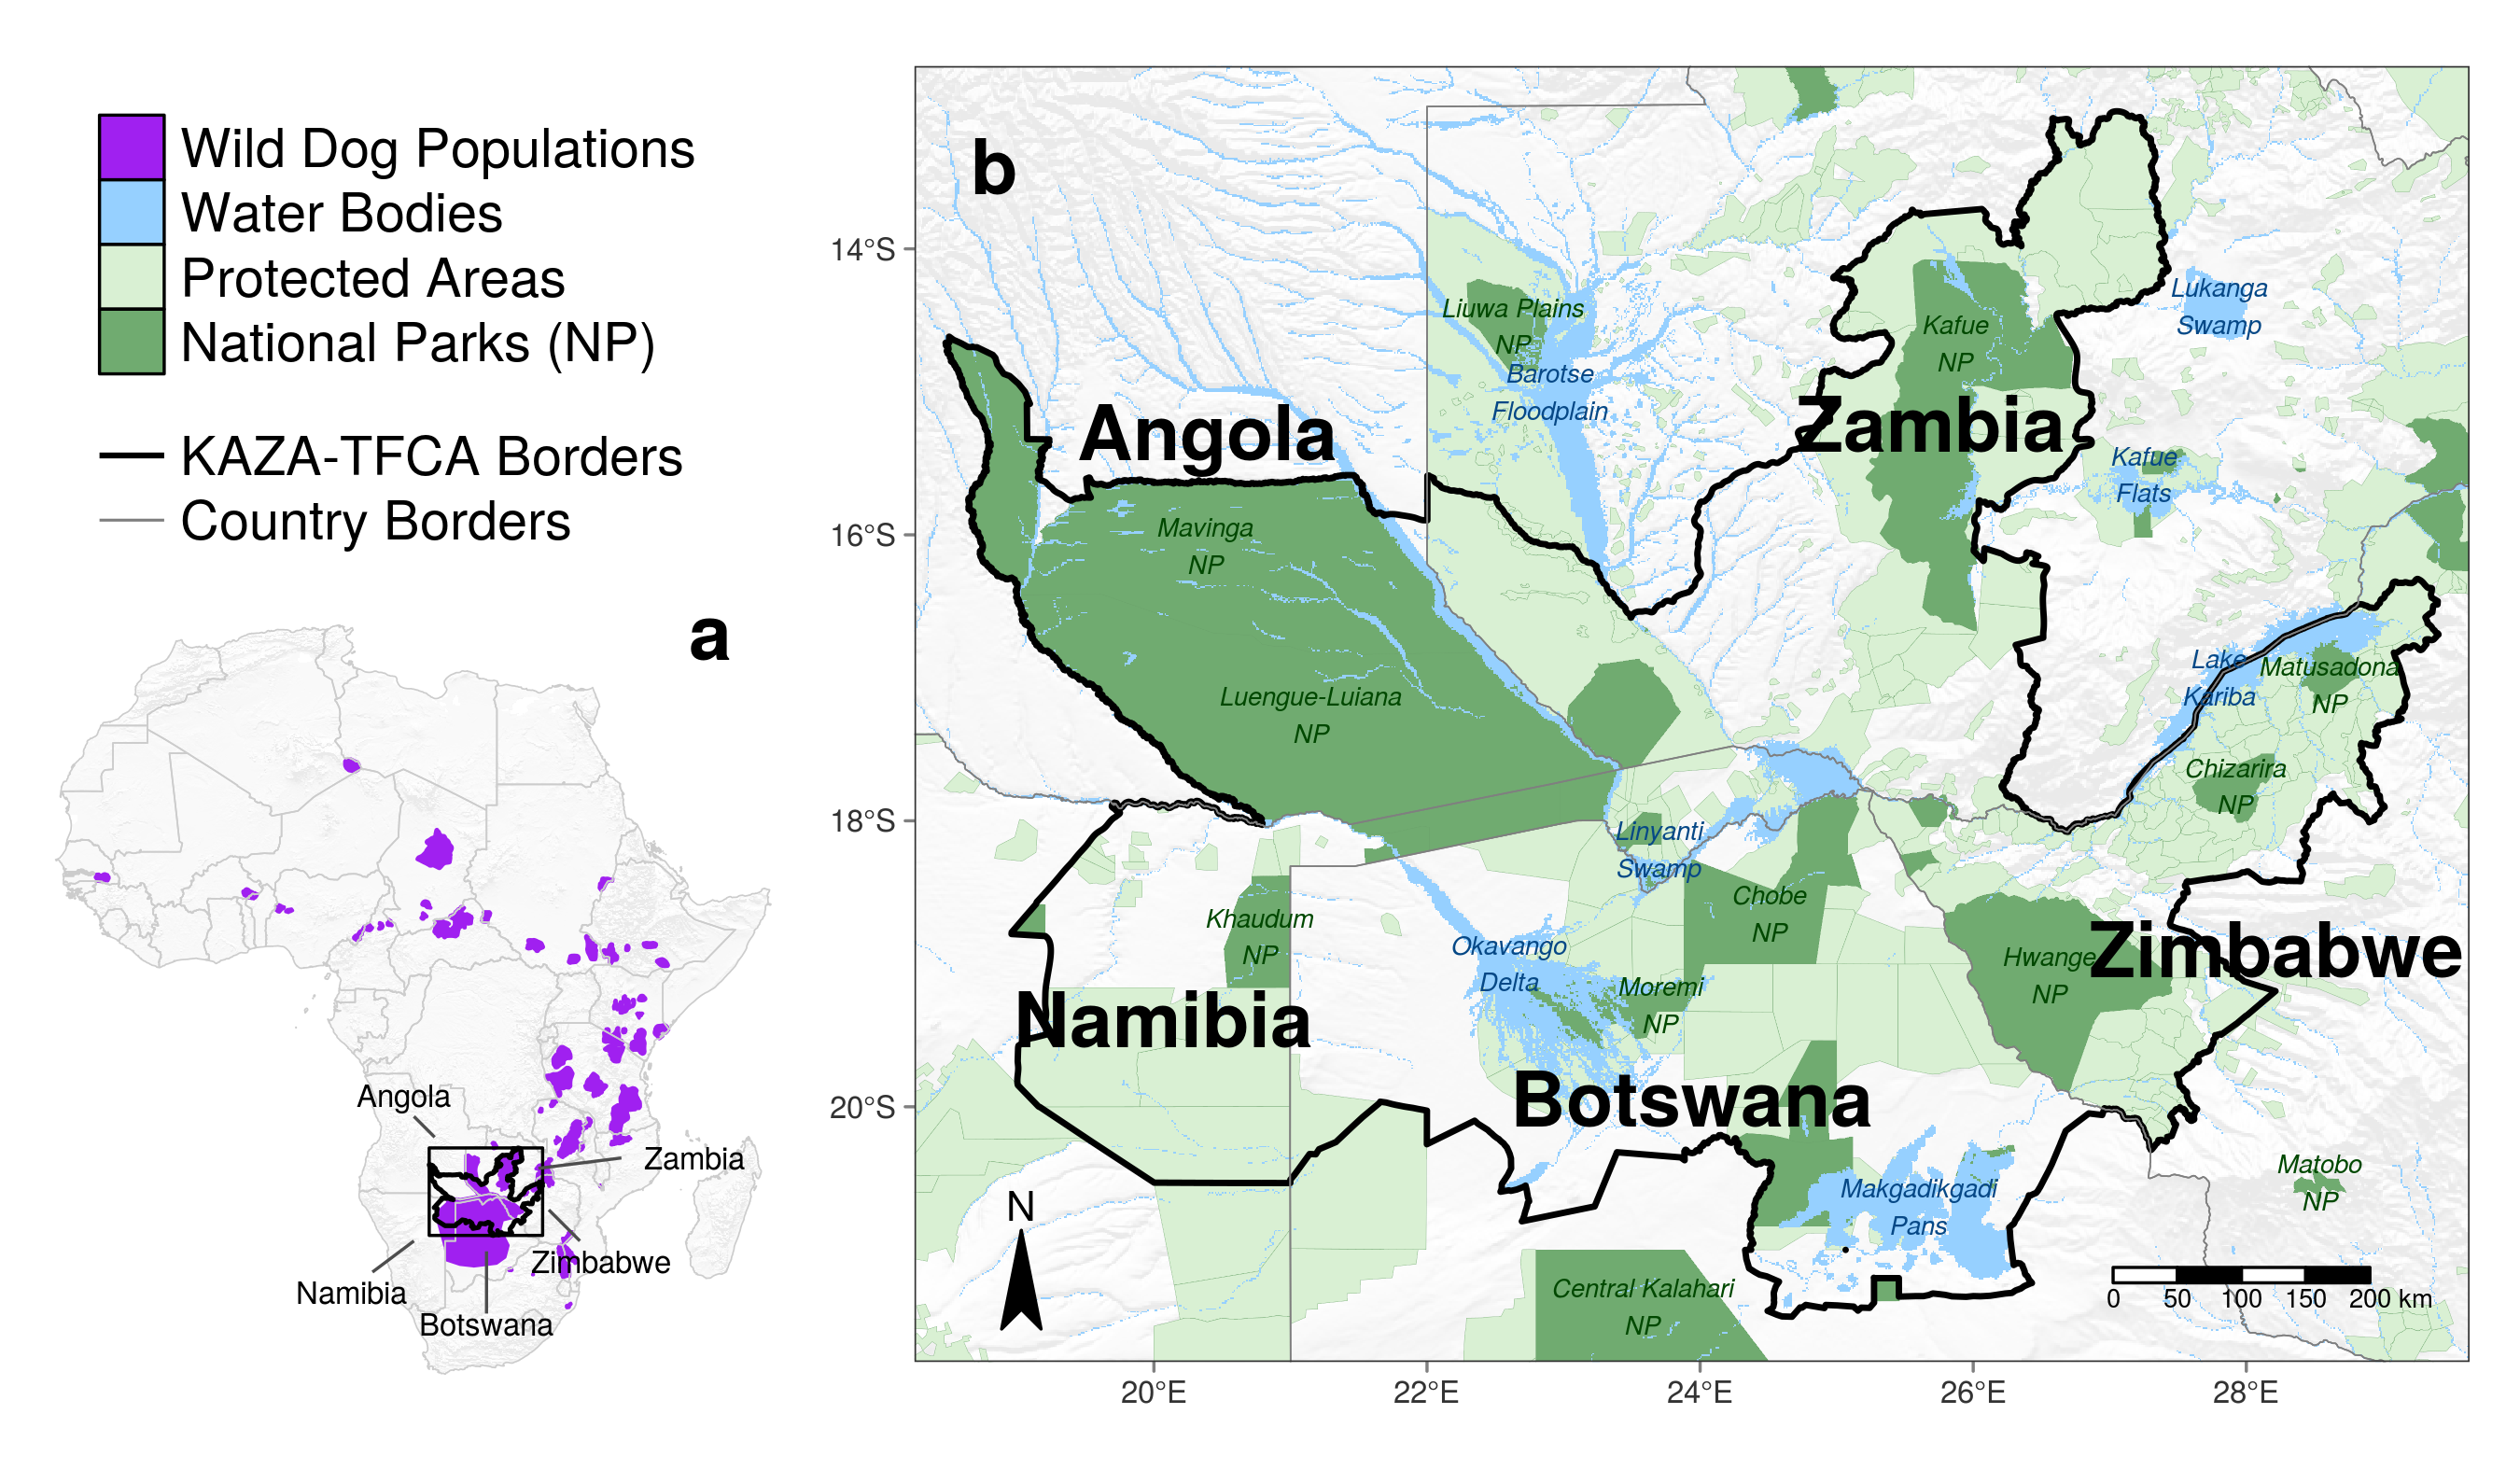
\includegraphics[width=\textwidth]{99_StudyArea.pdf}
        };
        \begin{scope}[x={(image.south east)},y={(image.north west)}]
            % % next four lines will help you to locate the point needed by forming a grid.
            % % comment these four lines in the final picture.
            % \draw[help lines,xstep=.1,ystep=.1] (0,0) grid (1,1);
            % \draw[help lines,xstep=.05,ystep=.05] (0,0) grid (1,1);
            % \foreach \x in {0,1,...,9} { \node [anchor=north] at (\x/10,0) {0.\x}; }
            % \foreach \y in {0,1,...,9} { \node [anchor=east] at (0,\y/10) {0.\y};}
            % % upto here
            \draw[black] (0.202, 0.255) -- (0.36, 0.955);
            \draw[black] (0.202, 0.205) -- (0.36, 0.070);
        \end{scope}
    \end{tikzpicture}
    \caption{Overview of our study area. (a) The red dotted rectangle depicts
    the study area, which was confined by a bounding box encompassing the entire
    KAZA-TFCA. Gray areas indicate remaining wild dog populations according to
    the IUCN \citep{Woodroffe.2012}. (b) The white rectangle illustrates the
    area within which dispersal coalitions were collared. Since Game Reserves in
    Botswana virtually serve the same purpose as National Parks, we use the
    terms interchangeably for this region.}
    \label{StudyArea}
  \end{center}
\end{figure}

\subsection{GPS Relocation Data}
We used a population of free-ranging African wild dogs inhabiting the Okavango
Delta in northern Botswana as a source population for dispersing individuals.
This population has been extensively studied since 1989 \citep{McNutt.1996,
McNutt.2008, Cozzi.2013, Cozzi.2020, Behr.2020}. Between 2011 and 2019, we
systematically collected GPS relocation data on 16 coalitions of dispersing
African wild dogs (7 female and 9 male coalitions; see also \cite{Abrahms.2017},
\cite{Cozzi.2020}, and \cite{Behr.2020}). Candidate dispersing individuals were
identified based on criteria reported in \cite{Behr.2020}, immobilized according
to protocols described in \cite{Osofsky.1996}, and fitted with GPS/Satellite
radio collars (\textit{Vertex Lite; Vectronic Aerospace GmbH, Berlin}) while
still in their natal pack. All procedures were undertaken and supervised by a
Botswana-registered wildlife veterinarian. Immobilized individuals were
monitored and all were observed to successfully re-join their packs within one
hour after immobilization. During dispersal, GPS collars were programmed to
record GPS relocation data every 4 hours and to regularly transmit them via
Iridium satellite system to a base station. The system thus allowed
remote-tracking of collared individuals, even where field conditions were
prohibitive or dispersal trajectories crossed international borders.

Because we were interested in dispersal behavior only, we discarded any GPS data
collected while individuals were still with their natal packs and also after
settlement in a new territory after dispersal \citep{Cozzi.2020}. We identified
the exact time of emigration and settlement based on direct field observations
and through visual inspection of the net squared displacement (NSD) metric. NSD
quantifies the euclidean distance of a relocation to a reference point
\citep{Borger.2012}, which in our case was the center of the dispersing
coalition's natal home range. Thus, dispersal was deemed to have started when a
coalition had left its natal home range and continued until the NSD metric
remained stationary, implying that the coalition had successfully settled
(Figure S1). Some coalitions undertook exploratory movements prior to proper
dispersal. Such movements have been observed in other species and are reported
to be very similar to proper dispersal \citep{Killeen.2014}. Therefore, we also
classified exploratory movements as dispersal. In total, we collected 4'169 GPS
relocations during dispersal, i.e. between emigration and settlement (Figure S2
\& Table S1), resulting in an average of 260 locations per dispersing coalition
(min = 37, max = 729). On average, coalitions dispersed for 48 days (min = 9,
max = 137), covered a mean euclidean distance of 54 km (min = 3, max = 263) and
a mean cumulative distance of 596 km (min = 130, max = 1'962). In our analysis,
we did not differentiate between male and female dispersing coalitions, for
previous research found little differences between sexes during dispersal
\citep{Woodroffe.2019, Cozzi.2020}.

\subsection{Spatial Covariates}
To investigate habitat preferences of dispersing wild dogs, we used a set of
geo-referenced covariates (\Cref{Covariates}) that we aggregated in the
categories \textit{land cover}, \textit{protection status}, and \textit{human
influence}. We did not include terrain features as covariates due to the absence
of noteworthy elevational gradients in our study area. For each covariate, we
prepared spatial raster layers from freely available online services or from
remotely sensed satellite imagery. To ensure a consistent resolution (i.e.
cell-size or grain) across covariates, we coarsened or interpolated all layers
to match a resolution of 250m x 250m. We performed processing and manipulation
of data as well as all spatial and statistical analyses using R, version 3.6.1
\citep{R.2019}.

\begin{figure}[h]
  \begin{center}
    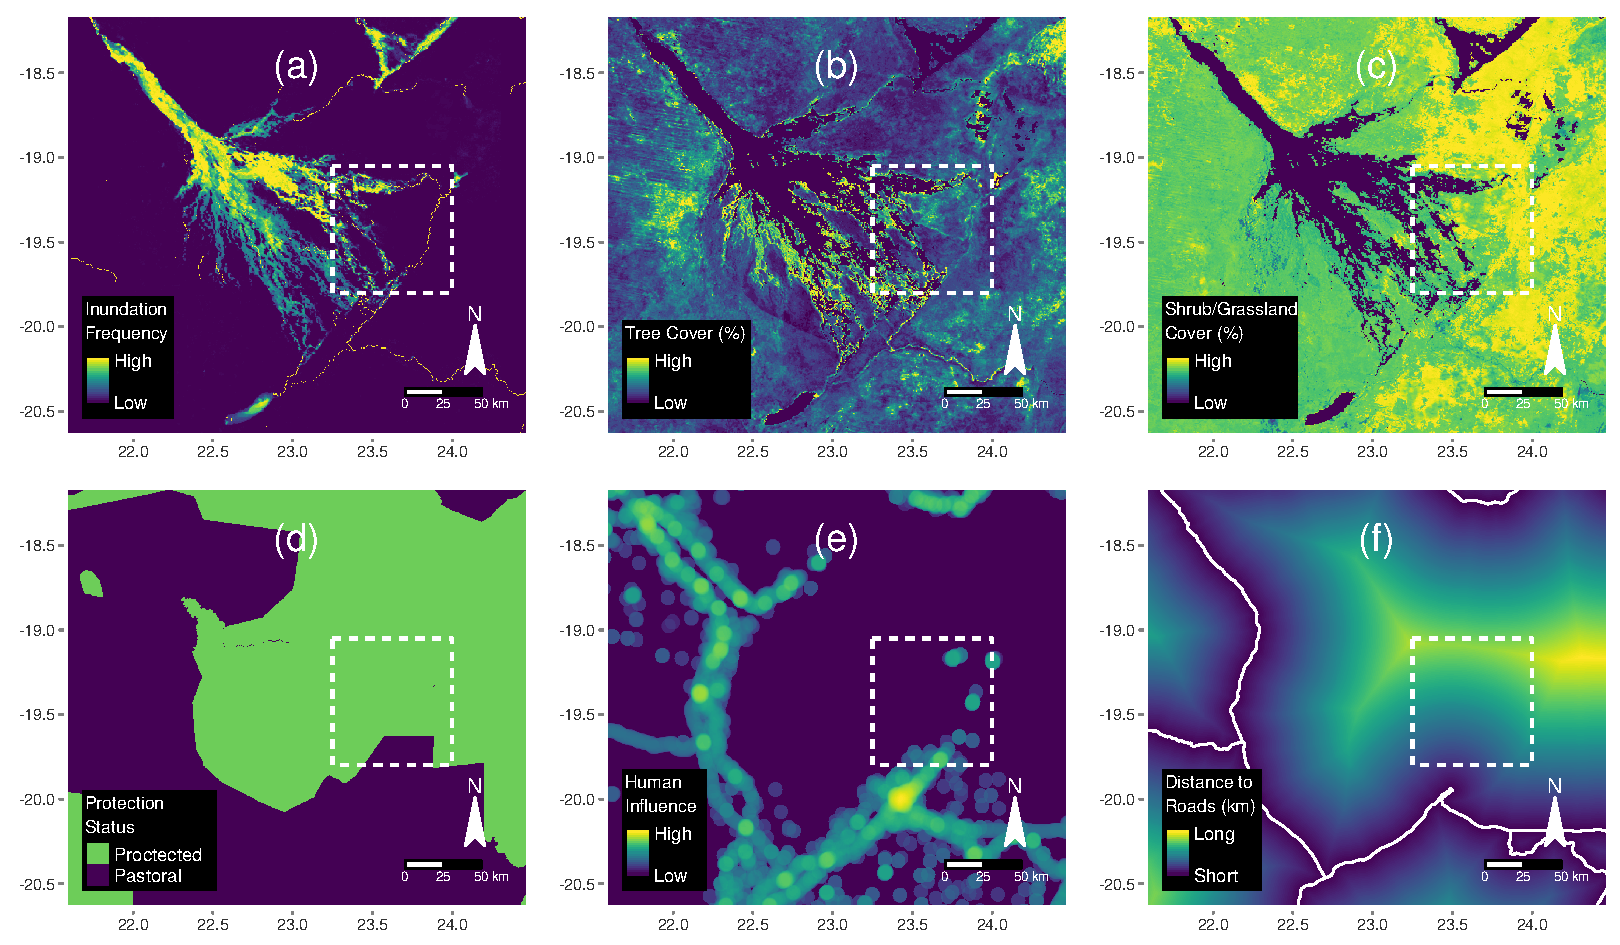
\includegraphics[width = \textwidth]{99_Covariates.pdf}
    \caption{Overview of spatial covariates that we included in our models. We
    prepared all covariates for the entire study area but for better visibility
    we only plot them for the surroundings of the Okavango Delta. The white
    rectangle in each plot depicts the area within which dispersal coalitions
    were collared. (a) Averaged layer of all dynamic (binary) water maps. (b)
    Percentage cover of trees. (c) Percentage cover of shrubs/grassland.
    Anything that was not covered by trees or shrubs/grassland was deemed to be
    bare land. (d) Protection status of the area. (e) Human influence proxy
    composed of human density, farms, and roads. (f) Distance to nearest road
    (white lines depict actual roads).}
    \label{Covariates}
  \end{center}
\end{figure}

\subsubsection{Land Cover}
We divided land cover into water and dryland. Water included rivers, wetlands,
and swamps. Because the inundation extent of the flood in the Okavango Delta is
highly variable within and between years, we created dynamic ``flood maps'' that
were updated every 8\textsuperscript{th} day following a remote sensing
algorithm developed by \cite{Wolski.2017}. The algorithm uses thresholding of
short wavelength infrared reflectances of MODIS Terra satellite imagery
(MCD43A4; \citealp{Schaaf.2015}) to distinguish areas covered by water and
dryland (details in Appendix A.3). While we created dynamic flood maps for the
Okavango Delta, we assumed the extent of all other water bodies (e.g. Chobe
river, Zambezi river) to be static within and between years. This static
representation was based on Globeland's land cover dataset \citep{Chen.2015},
from which we only retained the categories \textit{wetland} and \textit{water
bodies} and collectively reclassified them to \textit{water}. Globeland had an
original resolution of 30m x 30m, so we coarsened the layer to 250m x 250m using
the mode of each 250m x 250m cell. We further improved river representation by
employing the rasterized MERIT Hydro dataset \citep{Yamazaki.2019} from which we
added all rivers with a width of over 10m to our Globeland layer. We merged
dynamic and static water maps into a large rasterstack, covering the entire
study area. We also created a rasterstack rendering the covariate
\textit{distance to water} by calculating the eculidean distance of each raster
cell in the study area to the nearest source of water.

We further subdivided dryland into three layers as derived from the MODIS Terra
Vegetation Continuous Fields dataset (MOD44B; \citealp{Dimiceli.2015}). The
three layers depicted percentage cover of tree-vegetation (henceforth
\textit{trees}), non-tree-vegetation (henceforth \textit{shrubs/grassland}), and
non-vegetated (henceforth \textit{bare land}) and added up to 100\% of dryland
coverage. We used our flood map that aligned with the creation date of these
MODIS layers and defined anything covered by water as 0\% vegetated. The MODIS
vegetation layers had a resolution of 250m x 250m and no coarsening or
interpolation was required.

\subsubsection{Protection Status}
We created a binary layer separating protected from unprotected land. We
downloaded corresponding data on protection status in shapefile format from the
Peace Parks Foundation (\url{www.peaceparks.org}; \citealp{PeaceParks.2019}).
Protected areas included forest reserves, game reserves, wildlife management
areas, and national parks. We classified anything not covered by these
categories as unprotected (e.g. communal pastoral land, private land). We
rasterized the two categories to the binary raster \textit{protection status} (1
= protected, 0 = pastoral) with a resolution of 250m x 250m.

\subsubsection{Human Influence}
We created a raster layer representing human influence by integrating
information on (1) human density, (2) farming, and (3) roads.

\begin{enumerate}[label = (\arabic*)]

  \item We obtained spatial human density estimates through a publicly available
  30m x 30m high-resolution population density dataset
  (\url{www.dataforgood.fb.com}; \citealp{Facebook.2019}). We coarsened the
  layer to 250m x 250m by summing up human density values within each 250m x
  250m cell.

  \item We sourced spatial information on farms from the Globeland
  \citep{Chen.2015} and Cropland \citep{Xiong.2017} land cover datasets from
  which we retained areas that were classified as either \textit{cultivated
  land} or \textit{croplands}. Any other land cover class was not pertinent to
  farming and therefore omitted. Because both layers had a resolution of 30m x
  30m we coarsened them to 250m x 250m by assigning a value of 1 to any 250m x
  250m cell that covered farmland and a value 0 otherwise. Thus, the final layer
  depicted presence (= 1) or absence (= 0) of farms within each 250m x 250m
  cell.

  \item We obtained geo-referenced data on roads from Open Street Map
  \citep{OpenStreetMap.2019}, downloaded through Geofabrik
  (\url{www.geofabrik.de}). We only retained main tarmac roads and omitted
  smaller roads (Table S2) as these are scarcely frequented and do not represent
  an obstacle to wild dog movements \citep{Abrahms.2016}. We rasterized main
  tarmac roads to the binary raster \textit{roads} (1 = roads, 0 = no roads)
  with 250m x 250m resolution. Finally, we created the covariate
  \textit{distance to roads} by calculating the eculidean distance of each
  raster cell in the study area to the nearest road.

\end{enumerate}

\noindent Because layers (1), (2), and (3) depicted features that are typically
spatially clustered and because not all dispersing coalitions moved within
meaningful distance to each of these features, we totaled the layers
\textit{human density}, \textit{farming}, and \textit{roads}. This resulted in a
single covariate called \textit{human influence}. Note that totaling the layers
implied that the three covariates received different weights (see Appendix A.6
for details). To reduce the influence of outliers, totaled values were limited
to a maximum of 50, which visually resulted in a good balance between high and
low anthropogenic influence and was therefore considered appropriate for our
analysis. To render the fact that humans influence their surroundings beyond
their presence, we followed \cite{Elliot.2014} and applied to each raster cell a
5 km focal buffer within which we summed up and log-transformed human-influence
values (Figure S6).

\subsection{Habitat Selection Model}
We used an integrated step selection function (iSSF; \citealp{Avgar.2016}) to
investigate dispersers' selection or avoidance for the above-mentioned spatial
covariates. In the iSSF framework, GPS relocations are coerced to  ``steps'',
where a step is defined as the connecting line between two consecutive GPS
relocations \citep{Turchin.1998}. Subsequently, habitat preferences are
estimated by contrasting covariates along realized steps to the same covariates
along alternative ``random''  steps \citep{Fortin.2005, Thurfjell.2014,
Avgar.2016}. Thus, we paired each realized step with 24 random steps. We
generated random steps by sampling turning angles from a uniform distribution
U(\(-\pi, +\pi\)) and step lengths from a gamma distribution that was fitted
using realized steps \citep{Avgar.2016}. Together, a realized step and its 24
associated random steps formed a stratum of 25 steps that received a unique
identifier. Along all steps we extracted the above mentioned covariates (see
also Table S3). We also derived a binary covariate indicating whether or not a
step crossed a road and we identified the average distance of each step to the
nearest nearest road and the nearest source of water. We square-rooted the
values for \textit{distance to roads} and \textit{distance to water} to render a
decreasing marginal impact of distance. We standardized extracted values using a
z-score transformation, and checked for correlation using Pearson's Correlation
Coefficient \(r\). None of the covariates were overly correlated (\(|r| > 0.6\);
\citealp{Latham.2011}) and we retained all of them for modeling. Our habitat
selection model was then based on the assumption that dispersing wild dogs
assigned a selection score \(w(x)\) of the following exponential form to each
realized and random step \citep{Fortin.2005, Thurfjell.2014, Avgar.2016}:

\begin{equation}
\label{EQ1}
  w(x) = exp(\beta_1 x_1 + \beta_2 x_2 + ... + \beta_n x_n)
\end{equation}

\noindent The selection score \(w(x)\) of a step depended on its associated
covariates (\(x_1, x_2, ..., x_n\)), as well as on the animal's preferences for
these covariates (\(\beta_1, \beta_2, ..., \beta_n\)). To estimate habitat
preferences (i.e. the \(\beta\)'s) of interest, we used mixed effects
conditional logistic regression analysis as suggested by \cite{Muff.2020}. We
implemented their method using the R-package \textit{glmmTMB}
\citep{Mollie.2017} and used dispersing coalition ID to model random intercepts
and slopes. We defined two movement metrics, namely the cosine of the turning
angle (\(cos(ta)\)) and the log of the step length (\(log(sl)\)), as core
covariates and ran stepwise forward model selection based on Akaike's
Information Criterion (AIC; \citealp{Burnham.2002}) for all other covariates.
The inclusion of movement metrics served to reduce biases in estimated habitat
preferences that may have arised due to movement preferences \citep{Avgar.2016}.

To validate the predictive power of the most parsimonious habitat selection
model, we ran k-fold cross-validation for case-control studies as described in
\cite{Fortin.2009}. This validation procedure compares rank frequencies of
realized steps under observed and random preferences and proves a significant
prediction in case the confidence intervals of the spearman-rank correlation
coefficients \(\bar{r}_{s, realized}\) and \(\bar{r}_{s, random}\) do not
overlap (details in Appendix A.8).

\subsection{Permeability Surface}
Using the most parsimonious habitat selection model, we predicted a permeability
surface spanning the entire extent of the KAZA-TFCA. That is, we applied
\ref{EQ1} to our spatial covariates and calculated the selection score \(w(x)\)
for each raster cell in our study area. Because our flood maps were dynamic, we
collapsed all flood maps into a single static layer using areas that were
covered by water in at least 10\% of all our flood maps. We also calculated a
corresponding layer indicating the square-rooted euclidean distance of each
raster cell to the nearest source of water. To reduce the influence of outliers
in predicted permeability scores we followed \cite{Squires.2013} and curtailed
predicted scores between the 1\textsuperscript{st} and 99\textsuperscript{th}
percentile of their original values. To compare permeability across different
regions, we normalized the permeability surface to a range between 0 and 1. The
most impermeable landscape thus received a value of 0, the most permeable
landscape a value of 1. Based on the permeability surface we calculated median
permeability values within and outside the KAZA-TFCA, within and outside
formally protected areas, and within each of the five KAZA-TFCA countries.

\subsection{Least-Cost Paths and Corridors}
To identify movement corridors of dispersing wild dogs, we specified source
points and calculated factorial least-cost paths (LCPs) as well as factorial
least-cost corridors (LCCs) among all source points (Figure S.7;
\citealp{Adriaensen.2003, Sawyer.2011, Elliot.2014}). We generated source points
by overlaying the study area with a regular grid of points spaced at 100 km. We
only considered those points that fell within protected areas \(>\) 700
km\textsuperscript{2}, which conforms with home-range requirements of African
wild dogs reported in \cite{Pomilia.2015}. Finally, we defined centroids as
source points for those protected areas \(>\) 700 km\textsuperscript{2} that
were not assigned any source points from the regular grid. In total, we
generated 68 source points, which resulted in 2'278 unique pairwise combinations
and therefore 2'278 unique LCPs and LCCs.

We implemented factorial LCP analysis between source points using the R-package
\textit{gdistance} (Figure S.7; \citealp{vanEtten.2017}). The package translated
the (unscaled) permeability surface into a network of nodes to find shortest
effective distances between source points based on probabilities of moving from
cell to cell. In our case, the transition probability of moving between two
adjacent cells depended on their averaged permeability. We allowed individuals
to move from each cell to the cell's eight surrounding neighbors (i.e. Moores
neighborhood) and applied a geographic correction to account for the fact that
diagonal neighbors were more remote than orthogonal neighbors. Because African
wild dogs have been observed to cover large dispersal distances
\citep{DaviesMostert.2012, Masenga.2016, Cozzi.2020}, we did not limit LCPs to a
maximal effective cost. After computation, we tallied overlapping LCPs and
identified high-frequency routes.

We also calculated factorial LCCs \citep{Pinto.2009, Sawyer.2011, Elliot.2014},
again using the R-package \textit{gdistance} (Figure S.7;
\citealp{vanEtten.2017}). To identify LCCs, we first computed for each source
point a cumulative cost map, which indicated the total minimal costs required to
get from the source point to any other location in the study area. We then
obtained an LCC between two source points by adding up their cumulative cost
maps and masking out all cell-values exceeding the lowest cell-value by more
than 5\% \citep{Pinto.2009}. We repeated this procedure for each possible unique
pairwise combination of source points and thereby identified LCCs between all 68
selected source points. We normalized the resulting corridor-maps to range from
zero to one and tallied them into a single connectivity map.

\section{Results}
\subsection{Habitat Selection Model}
Our most parsimonious habitat selection model (\(\Delta AIC > 2\) than any
alternative model; Table S4) retained the covariates \textit{water},
\textit{distance to water}, \textit{trees}, \textit{shrubs/grassland}, and
\textit{human influence}, beside the fixed covariates \textit{cos(ta)} and
\textit{log(sl)} (\Cref{PermeabilityResults}a). Parameter estimates showed that
dispersing wild dogs moved in a directional and fast manner, as indicated by a
positive selection for small turning angles, i.e. high \(cos(ta)\) (\(\beta\) =
0.14; 95\% CI = 0.07 to 0.21, \Cref{PermeabilityResults}a) and longer steps,
i.e. high \(log(sl)\) (\(\beta\) = 0.06, 95\% CI = 0.02 to 0.09,
\Cref{PermeabilityResults}a). Dispersers avoided moving through water (\(\beta\)
= -0.52, 95\% CI -0.77 to -0.26, \Cref{PermeabilityResults}a) but selected for
locations in its vicinity, although the latter effect was not significant
(\(\beta\) = -0.32, 95\% CI = -0.72 to 0.08, \Cref{PermeabilityResults}a).
Dispersers avoided areas that were densely covered by trees (\(\beta\) = -0.31,
CI = -0.46 to -0.15, \Cref{PermeabilityResults}a) and preferred areas covered by
shrubs/grassland (\(\beta\) = 0.25, 95\% CI = 0.07 to 0.42,
\Cref{PermeabilityResults}a). Finally, dispersers avoided areas that were
influenced by human presence and activities (\(\beta\) = -0.41, 95\% CI = -0.78
to -0.05, \Cref{PermeabilityResults}a).

\begin{figure}[h]
  \begin{center}
    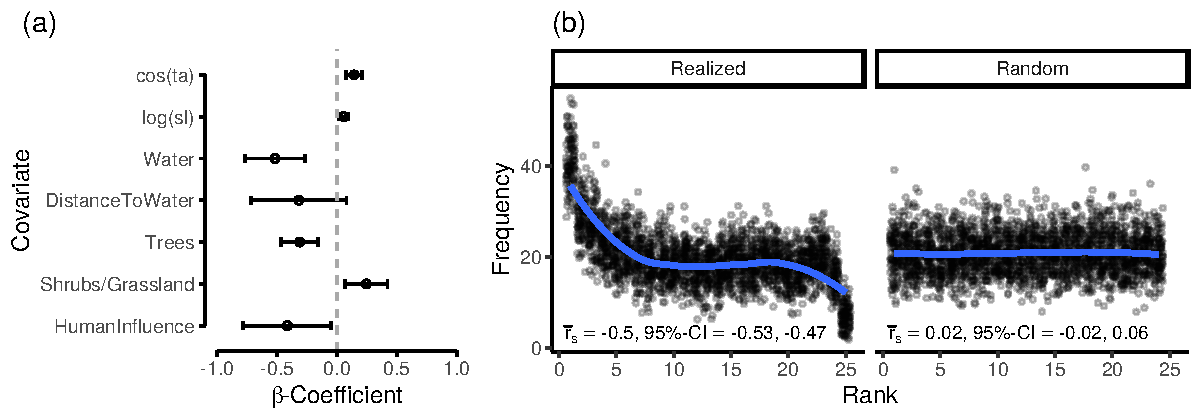
\includegraphics[width = \textwidth]{99_PermeabilityResults.pdf}
    \caption{(a) Estimated selection coefficients from the most parsimonious
    habitat selection model. Negative coefficients indicate avoidance of a
    covariate, positive coefficients selection of a covariate. Whiskers
    delineate the 95\%-CIs for estimated parameters. (b) Results from the k-fold
    cross validation for case-control studies. The left graph shows rank
    frequencies of \textit{realized} steps according to predictions, whereas the
    right graph shows rank frequencies of \textit{randomly selected} steps
    according to predictions. \(\bar{r}_s\) indicates the mean correlation
    coefficient resulting from 100 repetitions of the k-fold cross validation.
    The blue smoothing line was fitted using a locally weighted polynomial
    regression and serves to aid the eye in detecting the trends. Correlation
    coefficients suggest that our prediction was significant and robust,
    evidenced by the fact that the confidence intervals of \(\bar{r}_{s,
    realized}\) and \(\bar{r}_{s, random}\) did overlap and by the fact that
    there was strong and significant correlation between ranks and associated
    frequency for realized steps.}
    \label{PermeabilityResults}
  \end{center}
\end{figure}

Results from the k-fold cross-validation suggested that our prediction was
significant and robust, as highlighted by the fact that the 95\%-CIs intervals
of \(\bar{r}_{s, realized}\) and \(\bar{r}_{s, random}\) did not overlap
(\Cref{PermeabilityResults}b). Likewise, the significant correlation between
ranks and corresponding frequencies for realized steps suggested a good fit
between predictions and observations (\Cref{PermeabilityResults}b).

\subsection{Permeability Surface}
Our prediction of landscape permeability revealed substantial differences across
regions in the study area (\Cref{PermeabilityMap}). Comparisons of median
permeability values (\Cref{PermeabilityComp}) showed that permeability inside
KAZA-TFCA is more than two times as high as permeability outside it.
Permeability varies by country and reveals a five-fold permeability difference
among them. Angola and Botswana are characterized by comparably highly permeable
landscapes, Zimbabwe and Zambia are relatively impermeable, and Namibia ranges
in between the two extremes (\Cref{PermeabilityComp}). Visual inspection of our
covariate layers indicated that high permeability in Botswana and Angola is
mainly caused by a combination of low human presence and activities, low tree
cover, high shrubs/grassland cover, and a close distance to water. Although
swamps, wetlands, and permanent water themselves provide little permeability,
their surroundings act as strong attractants to dispersers. The low permeability
that characterizes Zambia and Zimbabwe, on the other hand, is mainly caused by
substantial human influences. Albeit the KAZA-TFCA covers a majority of
permeability hot-spots, several highly permeable regions remain uncovered by its
borders. Across all countries, protected areas provide roughly double the
permeability of human-dominated landscapes (\Cref{PermeabilityComp}).

\begin{figure}[hbtp]
  \begin{center}
    \begin{tikzpicture}
        \node[anchor=south west,inner sep=0] (image) at (0,0,0) {
          \begin{minipage}{\textwidth}
            \includegraphics[width = \textwidth]{99_PermeabilityMap.pdf}
          \end{minipage}
        };
        \begin{scope}[x={(image.south east)},y={(image.north west)}]
        \end{scope}
    \end{tikzpicture}
    \caption{Predicted permeability surface for the extent of the KAZA-TFCA.
    Permeability was predicted by calculating selection scores \(w(x) =
    exp(\beta_1 x_1 + \beta_2 x_2 + ... + \beta_n x_n)\) for each raster cell
    based on the raster cell's underlying covariates (\(x_i\)) and estimated
    habitat preferences (\(\beta_i\)). Areas that dispersers find easy to
    traverse are depicted in bright colors. Bold white lines delineate the
    borders of the KAZA-TFCA, whereas dashed white lines show country borders.}
    \label{PermeabilityMap}
  \end{center}
\end{figure}

\begin{table}[h]
  \begin{center}
  \caption{Comparison of median permeability (interquantile range in brackets)
  across countries, separated into areas within and outside the KAZA-TFCA, as
  well as within and outside formally protected areas. High values indicate high
  permeability, whereas low values correspond to low permeability.}
  \label{PermeabilityComp}
  \begin{tabular}{llllll}
    \toprule
    \multicolumn{1}{c}{} & \multicolumn{2}{c}{KAZA-TFCA} &
    \multicolumn{2}{c}{Protection Status} & \multicolumn{1}{c}{} \\
    \cmidrule(l{3pt}r{3pt}){2-3} \cmidrule(l{3pt}r{3pt}){4-5}
    Country & Inside & Outside & Protected & Pastoral & Overall\\
    \midrule
    Angola & 0.36 (0.41) & 0.12 (0.32) & 0.36 (0.41) & 0.12 (0.33) & 0.20 (0.39)\\
    Botswana & 0.25 (0.30) & 0.15 (0.16) & 0.28 (0.35) & 0.15 (0.18) & 0.19 (0.25)\\
    Namibia & 0.22 (0.30) & 0.13 (0.18) & 0.24 (0.30) & 0.11 (0.15) & 0.16 (0.24)\\
    Zambia & 0.05 (0.09) & 0.03 (0.06) & 0.04 (0.10) & 0.03 (0.05) & 0.03 (0.07)\\
    Zimbabwe & 0.07 (0.16) & 0.06 (0.05) & 0.08 (0.17) & 0.05 (0.05) & 0.06 (0.07)\\
    \hline
    Overall & 0.16 (0.30) & 0.07 (0.15) & 0.15 (0.30) & 0.07 (0.15) & 0.10 (0.22)\\
    \bottomrule
  \end{tabular}
  \end{center}
\end{table}

\subsection{Least-Cost Paths \& Least-Cost Corridors}
Our least-cost analysis revealed three major movement corridors of which all
were well-within the KAZA-TFCA boundaries (\Cref{LeastCost}). Furthermore, we
found little to no direct connectivity between peripheral points; that is, most
paths and corridors connecting two adjacent peripheral points run through more
central regions before heading towards their destination at the periphery
(\Cref{LeastCost}). One major corridor runs SE-NW and connects the
Okavango-Linyanti ecosystem in Botswana with Luengue-Luiana NP in Angola. A
second corridor runs W-E between Chobe NP in Botswana and Zimbabwe's Hwange NP.
A third major corridor runs NE-SW, completely across unprotected areas, and
connects Kafue NP in Zambia with more central regions of the KAZA-TFCA. Several
minor corridors branch off from these three major corridors; these include a
southward connection between the Okavango-Linyanti and the Central Kalahari Game
Reserve, a southwesterly corridor connecting Luengue-Luiana NP with Namibia's
Kaudom NP, and a northeasterly extension of the Hwange corridor into Zimbabwe's
Matusadona NP. According to our predictions, the corridor towards Kafue NP and
the corridor passing the Okavango-Linyanti region are the highest frequented
routes within the KAZA-TFCA (\Cref{LeastCost}, dark red colors). Our model did
not detect any significant direct corridors between Zimbabwe and Zambia or
Zambia and Angola, and only a very limited W-E direct connection between the
Okavango region and Namibia's Khaudum NP. Except for the corridor into the
Central Kalahari National Park, our model did not detect any significant
connectivity outside the boundaries of the KAZA-TFCA.

\begin{figure}[hbtp]
  \begin{center}
    \begin{minipage}{0.95\textwidth}
      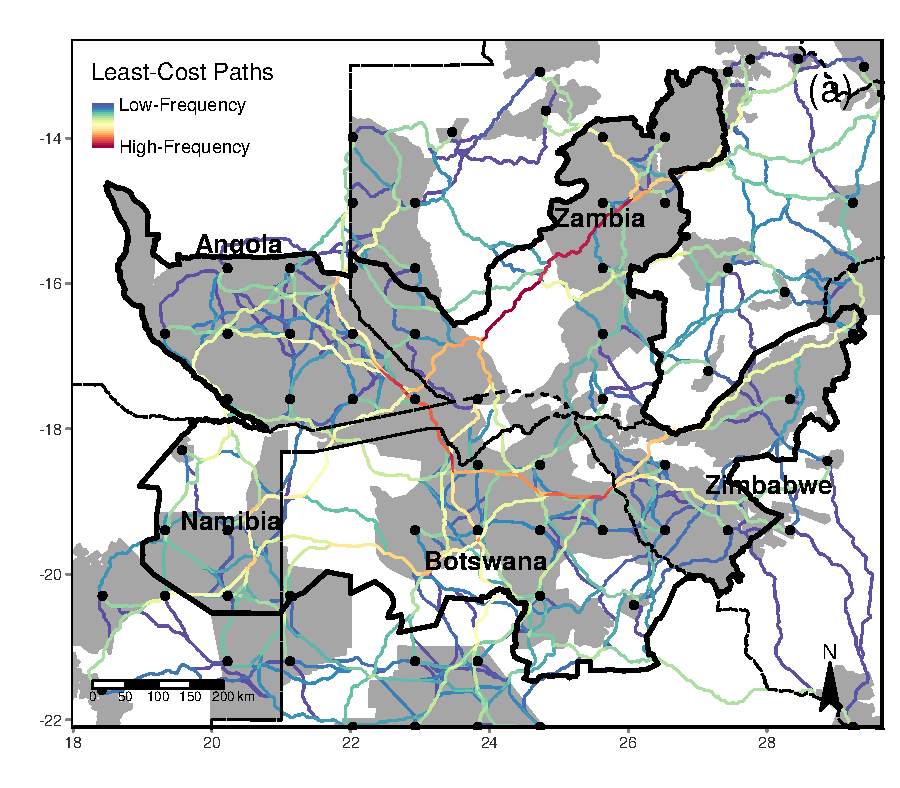
\includegraphics[width = 0.95\textwidth]{99_LeastCostPaths.pdf}
      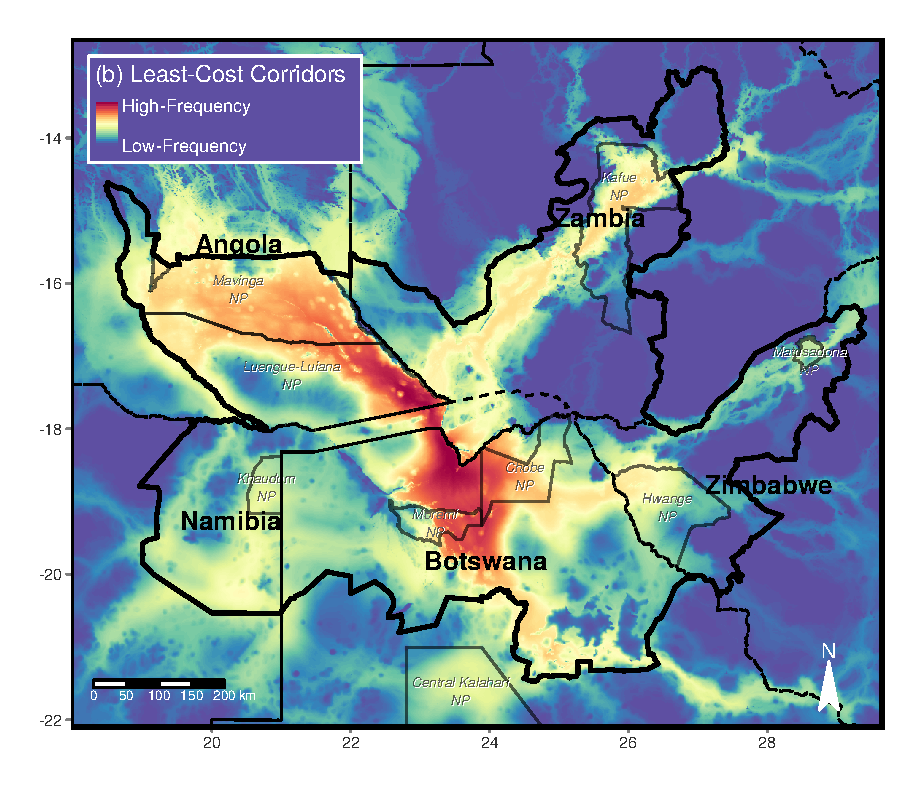
\includegraphics[width = 0.95\textwidth]{99_LeastCostCorrs.pdf}
    \end{minipage}
    \caption{(a) Source points (black dots) and corresponding least-cost paths
    leaving from protected areas (light grey). Note that only contiguous
    protected areas covering more than 700 km\textsuperscript{2} are depicted.
    Continuous thin black lines indicate the borders of the KAZA-TFCA, whereas
    dashed black lines delineate country-borders. (b) Least-cost corridors
    between the same source points as illustrated in subfigure (a). For ease of
    spatial reference, we also labeled some national parks (dark-grey).}
    \label{LeastCost}
  \end{center}
\end{figure}

\section{Discussion}
We used GPS relocation data collected on dispersing African wild dogs to
investigate whether their main movement corridors are contained within the
boundaries of the world's largest transboundary conservation area, namely the
KAZA-TFCA. Our analysis suggests that the KAZA-TFCA indeed encompasses all major
movement corridors of African wild dogs, demonstrating the potential value of
such an initiative. We thus expemplified how pertinent dispersal data of a
highly mobile species can be used to assess the adequacy of already existing or
planned protected areas. Our approach is neither limited to the African wild
dog, nor to our study area. All covariates used throughout this study are
readily available on a global scale and many of them are likely to be important
determinants of movement behavior, landscape permeability, and connectivity for
other species \citep{Thurfjell.2014, Zeller.2012}. Interestingly, our predicted
network of least cost-paths and corridors for African wild dogs shows surprising
similarities to corridors of dispersing lions inhabiting the same ecosystem
\citep{Elliot.2014, Cushman.2018}. This not only reinforces confidence in our
own predictions but also suggests potential synergies for the conservation of
these two, and possibly more, species. Expanding this analytical framework to
additional species will yield important insights on the consistency of
inter-specific movement corridors, thus highlighting areas that are
exceptionally valuable for the conservation of several species.

Locally, we identified the Okavango-Linyanti region as a potential dispersal hub
through which dispersersing wild dogs gain access to more peripheral regions of
the KAZA-TFCA. While this might partly be owed to the area's central position
within our study area, it is likely also due to its unique environmental and
anthropogenic characteristics. It appears that the absence of human activities
and the presence of relatively impermeable water bodies, such as the Okavango
Delta and the Linyanti Swamp funnel dispersal movements, resulting in a highly
frequented corridor. The region is also instrumental for connecting wild dog
subpopulations in Zambia's Kafue and Zimbabwe's Hwange NPs
\citep{Woodroffe.2012}. These subpopulations are currently separated by the
Zambezi River, forcing dispersers to detour via northern Botswana to reach more
peripheral areas. The key role of the Okavango-Linyanti region for overall
connectivity within the KATA-TFCA thus calls for actions to secure its
protection status in the future. While the region is currently a Wildlife
Management Area devoted to photographic tourism, it has neither the status of a
National Park nor that of a Game Reserve and so potentially faces growing
pressure towards exploitation of its natural resources under the influences of
an expanding human population, farming, and cropping industry. A similar case of
non-formally protected but key dispersal landscape is represented by the area
south of Kafue NP in Zambia, for which a disruption of its main and narrow
dispersal corridor would result in considerable isolation of its subpopulations.
We also revealed a potential southwards corridor between the Okavango-Linyanti
ecosystem and the Central Kalahari National Park. \cite{Elliot.2014} and
\citep{Cushman.2018} identified a similar corridor for dispersing lions,
suggesting that upholding and protecting a link between those ecosystems is
pivotal. Some areas through which the corridor runs are neither part of the
KAZA-TFCA nor profit from any form of protected status. In fact, human presence
and activities along the national road that longitudinally traverses this
corridor may limit realized connectivity \citep{Cozzi.2020}. Finally, our
connectivity map suggested that connectivity within the extent of the KAZA-TFCA
gradually decreases towards the borders of our study area, yet this might partly
be a result of boundary effects \citep{Koen.2010}.

Our approach of identifying movement corridors based on pre-defined start and
end points implicitly assumes that individuals know the end point of their
dispersal journey and that they have almost complete knowledge of associated
movement costs \citep{Panzacchi.2016}. Since dispersers often move into unknown
territory, this may not necessarily be the case \citep{Abrahms.2017,
Woodroffe.2019, Cozzi.2020}. However, specification of pre-defined end points
might not be necessary, as the parametrized iSSF model can be applied as a
mechanistic movement model to simulate dispersal events from known source
points, yet without restricting the domain of potential end points
\citep{Signer.2017}. Consequently, movement corridors would emerge more
naturally as the result of a myriad of simulated dispersal events. An approach
that does not require the creation of end points will also be instrumental in
identifying corridors outside formally protected areas. In contrast to classical
corridor mapping, individual-based movement simulations would further allow
considering movement preferences of dispersers as well as rendering the temporal
aspect of dispersal (for instance to examine how quickly dispersers are able to
move between locations). The latter consideration is particularly important in
ecosystems where connectivity may change in response to seasonal variations in
the landscape \citep{Osipova.2019}. While a simulation based approach is
conceptually straightforward, it requires a comprehensive mechanistic
understanding of dispersal movements, which is conditional on our ability to
collect additional dispersal data and adequately represent the landscape through
which individuals disperse.

Our results further emphasize that human presence and activities constitute some
of the main barriers to connectivity. Our result that human influence is
detrimental to dispersal conforms to findings on dispersing wild dogs from
eastern Africa \citep{Masenga.2016, Oneill.2020} but conflicts with findings by
\cite{DaviesMostert.2012}, who reported a comparably high willingness of
dispersers to cross human-dominated landscapes in South Africa. We believe that
such differences are due to the unavailability of alternative ``natural''
routes, which may have forced dispersers in South Africa to cross human
dominated landscapes despite a strong aversion to do so. These contrasting
findings may hint at a considerable ability of dispersing wild dogs to adapt to
prevailing habitat conditions (see e.g. \cite{Woodroffe.2011}) and could imply a
limited model transferability between dispersersers from our study system to
dispersers found in other ecosystems, such as in South Africa
\citep{Whittington.2011, DaviesMostert.2012} or Kenya \citep{Woodroffe.2019,
Oneill.2020}. However, we believe that our study population adequately
represents wild dog populations residing within the greater extent of the
KAZA-TFCA, where more natural dispersal routes are readily available. Successful
conservation of this species is thus strictly contingent on policymakers' and
local authorities' willingness and ability to provide and conserve areas that
remain free from anthropogenic pressures. This is not only paramount in light of
providing connectivity and facilitating dispersal, but also in terms of reducing
human-caused mortality during dispersal. In fact, previous studies have shown
that human-caused mortality during dispersal, especially in proximity to
settlements and roads, represents a major threat to the dispersal ability of
this species \citep{Woodroffe.2019, Cozzi.2020}.

Besides anthropogenic pressures, we identified water as another major obstacle
to dispersal. This corroborates earlier studies which showed that water bodies
(including swamps) are almost impenetrable by resident packs
\citep{Abrahms.2017, Cozzi.2020} and only infrequently crossed by dispersing
individuals \citep{Cozzi.2020}. An accurate and dynamic representation of water
is thus imperative and particularly relevant in seasonal or flood-pulsing
ecosystems such as the Okavango Delta. In fact, future studies could investigate
how connectivity across such systems changes in result to seasonal changes in
the environment (see also \cite{Osipova.2019}).

Although dispersers avoided moving through water, we revealed a preference for
moving in proximity to water. This preference is likely explained by high
prey-availability in vicinity of water \citep{Western.1975, Bonyongo.2005}.
However, following the same reasoning, apex predators (e.g. lions, spotted
hyenas) and resident wild dogs may prefer proximity to water
\citep{Valeix.2010}, thereby occasionally forcing dispersing wild dogs into
prey-poorer areas that are more distant to water \citep{Ndaimani.2016} and pose
a lower risk of aggressive intraguild interactions \citep{Creel.1996,
Mills.1997, Webster.2012}. We could not control for the presence or absence of
apex predators or conspecifics during dispersal as we lacked corresponding data,
but these considerations may explain why we did not find a significant effect of
\textit{distance to water}. Given the influence that resident conspecifics,
predators, competitors, and prey can have on dispersers \citep{Cozzi.2018,
Armansin.2019} future studies should strive to collect and incorporate
corresponding ``social'' information into analyses of landscape connectivity to
more precisely reconstruct dispersal corridors.

\section{Conclusion}
Our work shows how dispersal data of a highly mobile species can be used
identify movement corridors and assess the adequacy of protected areas. In our
case, the predicted dispersal corridors of African wild dogs were well contained
within the boundaries of the world's largest transboundary conservation area,
namely the KAZA-TFCA, suggesting that it will significantly contribute to the
long-term viability of this species. Moreover, our connectivity network allowed
to reveal potential dispersal hubs thorugh which dispersers gain access to more
remote regions in the study area. Finally, our investigations showed that human
influence constitutes one of the main barriers to dispersal and substantially
reduces landscape connectivity accross large scales. Successful conservation of
wide-ranging species, such as exemplified by the African wild dog, will
therefore be contingent on the willingness of local authorities, policymakers,
and land managers to preserve areas that remain free from human strains.
Ultimately, our work contributes to the growing field of connectivity literature
and provides and easily expandible framework for the assessement of existing or
planned protected areas.

\section{Author's Contributions}
D.D.H., D.M.B., and G.C. conceived the study and designed methodology; D.M.B.,
G.C., and J.W.M. collected the data; D.D.H. and D.M.B. analysed the data; G.C.
and A.O. assisted with modelling; D.D.H., D.M.B., and G.C. wrote the first draft
of the manuscript and all authors contributed to the drafts at several stages
and gave final approval for publication.

\section{Data Availability}
GPS movement data of dispersing coalitions will be made available on dryad at
the time of publication.

\section{Acknowledgements}
We thank the Ministry of Environment and Tourism of Botswana for granting
permission to conduct this research. We thank C. Botes, I. Clavadetscher, and G.
Camenisch for assisting with wild dog immobilizations. We also thank B. Abrahms
for sharing her data of three dispersing wild dogs. Furthermore, we are indebted
to Prof. J. Fieberg, who consulted all statistical aspects of this work and P.
Wolski, from the Okavango Research Institute, who assisted us in generating
dynamic flood maps. This study was funded by Basler Stiftung für Biologische
Forschung, Claraz Foundation, Idea Wild, Jacot Foundation, National Geographic
Society, Parrotia Stiftung, Stiftung Temperatio, Wilderness Wildlife Trust
Foundation, Forschungkredit der Universität Zürich, and a Swiss National Science
Foundation Grant (31003A\_182286) to A. Ozgul.

\newpage
\begingroup
\singlespacing
\bibliography{Literatur}
\endgroup

\end{document}
